\documentclass[10pt]{article}
%----------Packages----------
\usepackage[utf8]{inputenc}
\usepackage[landscape,left=5mm,right=5mm,top=5mm,bottom=5mm]{geometry}
\usepackage{amsmath,amssymb}
\usepackage{siunitx}
\usepackage{multicol}
\usepackage{blindtext}
\usepackage{graphicx}

\usepackage[shortlabels]{enumitem}
\setlist[enumerate]{topsep=0pt,noitemsep}
\setlist[enumerate,1]{label=\arabic*.}

%----------Page formatting----------
\pagenumbering{gobble}
\setlength{\parindent}{0pt}
\newcommand{\tablewidth}{0.48\textwidth}

%----------Symbols----------
\newcommand{\Z}{\mathbb Z}
\newcommand{\R}{\mathbb R}
\newcommand{\C}{\mathbb C}

\newcommand{\om}{\omega}
\newcommand{\al}{\alpha}
\newcommand{\be}{\beta}
\newcommand{\ze}{\zeta}

\newcommand{\Om}{\Omega}

%----------Brackets----------
\newcommand{\lrb}[1]{\left(#1\right)}
\newcommand{\agb}[1]{\left\langle#1\right\rangle}
\newcommand{\sqb}[1]{\left[#1\right]}
\newcommand{\set}[1]{\left\{#1\right\}}
\newcommand{\abs}[1]{\left|#1\right|}

\let\originalleft\left
\let\originalright\right
\renewcommand{\left}{\mathopen{}\mathclose\bgroup\originalleft}
\renewcommand{\right}{\aftergroup\egroup\originalright}

%----------Differentiation----------
\renewcommand{\d}{\,d}
\newcommand{\dv}[2]{\frac{d#1}{d#2}}
\newcommand{\ddv}[2]{\frac{d^2#1}{dt^2}}

%----------Integration----------
\newcommand{\infint}{\int_{-\infty}^{\infty}}
\newcommand{\infsum}{\sum_{k=-\infty}^{\infty}}
\newcommand{\ksum}{\sum_{k=0}^{N-1}}
\newcommand{\nsum}{\sum_{n=0}^{N-1}}

%----------General----------
\newcommand{\ds}{\displaystyle}
\newcommand{\ts}{\textstyle}
\newcommand{\tab}{\hspace{.02\textwidth}}
\newcommand{\oneEqn}[2]{$\makebox[#2][l]{$#1$}$}
\newcommand{\twoEqn}[4]{$\makebox[#3][l]{$#1$} \makebox[#4][l]{$#2$}$}
\newcommand{\threeEqn}[6]{$\makebox[#4][l]{$#1$} \makebox[#5][l]{$#2$} \makebox[#6][l]{$#3$}$}
\newcommand{\fourEqn}[8]{$\makebox[#5][l]{$#1$} \makebox[#6][l]{$#2$} \makebox[#7][l]{$#3$} \makebox[#8][l]{$#4$}$}
\newcommand{\splittab}{\hspace{2.58ex}}

%----------Sections----------
\makeatletter
\renewcommand{\section}{\@startsection{section}{1}{0ex}{-1ex}{0.7ex}
                        {\normalfont\large\bfseries}}
% \renewcommand{\subsection}{\@startsection{subsection}{2}{0ex}{-0.4ex}{0.4ex}
%                         {\normalfont\normalsize\bfseries}}
\renewcommand{\subsection}{\@startsection{subsection}{2}{0ex}{-0.4ex}{0.4ex}
                        {\normalfont\normalsize\underline}}
\makeatother
\setcounter{secnumdepth}{0}

%----------ELEC 221----------
\newcommand{\stretchamt}{1.2}
\newcommand{\F}{\mathcal{F}}
\renewcommand{\L}{\mathcal{L}}
\newcommand{\ft}{\overset{\mathcal{F}}{\longleftrightarrow}}
\newcommand{\lt}{\overset{\mathcal{L}}{\longleftrightarrow}}
\renewcommand{\Re}{\text{Re}}
\renewcommand{\Im}{\text{Im}}
\newcommand{\phase}{\sphericalangle}
\renewcommand{\Re}{\text{Re}}
\renewcommand{\Im}{\text{Im}}
\newcommand{\ROC}{\text{ROC}}

%----------Document Begins Here----------
\begin{document}

\begin{multicols*}{3}
\raggedcolumns

{\LARGE{\underline{ELEC 221 Formula Sheet}}}

\section{Signals Basics}

{\renewcommand{\arraystretch}{\stretchamt}
\begin{tabular}{@{}ll}
    DT signals & $x[n], n\in\Z$ \\
    CT signals & $x(t), t\in\R$ \\
    IV transformation & $x(t)\to x(\alpha t+\be)$ \\
    & 1. Shift by $\be$ \\
    & 2. Compress by $\abs{\alpha}$ \\
    & 3. Reverse if $\alpha<0$ \\
    Periodic, period $T$ & $x(t+T)=x(t)$ \\
    Odd & $x(-t)=-x(t)$ \\
    Even & $x(-t)=x(t)$
\end{tabular}}

\section{Systems Basics}

{\renewcommand{\arraystretch}{\stretchamt}
\begin{tabular}{@{}ll}
    DT systems & $x[n]\to y[n]$ \\
    CT systems & $x(t)\to y(t)$
\end{tabular}}

{\renewcommand{\arraystretch}{\stretchamt}
\begin{tabular}{@{}ll}
    1. Memoryless & $y(t_0)$ depends only on $x(t_0)$ \\
    2. Invertible & distinct $x(t)$ map to distinct $y(t)$ \\
    3. Causal & $y(t_0)$ depends only on $x(t)$ for $t\leq t_0$ \\
    4. Stable & bounded input $\implies$ bounded output \\
    5. Linear & $ax_1(t)+bx_2(t)\to ay_1(t)+by_2(t)$ \\
    6. \rlap{Time-invariant} & \hspace{4ex}$x(t-t_0)\to y(t-t_0)$
\end{tabular}}

\section{DT Impulse and Convolution Sum}

{\renewcommand{\arraystretch}{\stretchamt}
\begin{tabular}{@{}ll}
    DT unit impulse & $\delta[n]=\begin{cases}1 & n=0 \\ 0 & n\neq 0\end{cases}$ \\
    DT unit step & $u[n]=\begin{cases}1 & n\geq 0 \\ 0 & n<0\end{cases}$ \\
    Relations & $\delta[n]=u[n]-u[n-1]$ \\
    & $u[n]=\sum_{m=0}^\infty\delta[n-m]=\sum_{k=-\infty}^n\delta[k]$ \\
    Sampling & $x[k]=x[n]\delta[n-k]$ \\
    Weighted sum & $x[n]=\infsum x[k]\delta[n-k]$ \\
    Impulse response & $\delta[n-k]\to h_k[n]$ \\
    & $y[n]=\infsum x[k]h_k[n]$ \\
    Time-invariant & $\delta[n]\to h[n]$ \\
    & $\delta[n-k]\to h[n-k]$ \\
    Convolution & $y[n]=\infsum x[k]h[n-k]$ \\ 
    & $y[n]=x[n]*h[n]$
\end{tabular}}

\subsection{Convolution Properties}

{\renewcommand{\arraystretch}{\stretchamt}
\begin{tabular}{@{}ll}
    Associative & $x[n]*(h_1[n]*h_2[n])$ \\ 
    & $=(x[n]*h_1[n])*h_2[n]$ \\
    Commutative & $x[n]*h[n]=h[n]*x[n]$ \\
    Distributive & $x[n]*(h_1[n]+h_2[n])$ \\
    & $=x[n]*h_1[n]+x[n]*h_2[n]$
\end{tabular}}

\section{CT Impulse and Convolution Integral}

{\renewcommand{\arraystretch}{\stretchamt}
\begin{tabular}{@{}ll}
    CT unit impulse & $\delta(t)=\begin{cases}\infty & t=0 \\ 0 & t\neq 0\end{cases}$ \\
    & $\infint\delta(\tau)\d\tau=1$ \\
    CT unit step & $u(t)=\begin{cases}1 & t\geq 0 \\ 0 & t<0\end{cases}$ \\
    Relations & $\delta(t)=\dv{u(t)}{t}$ \\
    & $u(t)=\int_{-\infty}^t\delta(\tau)\d\tau$ \\
    Weighted integral & $x(t)=\infint x(\tau)\delta(t-\tau)\d\tau$ \\
    Impulse response & $\delta(t)\to h(t)$ \\
    Convolution & $y(t)=\textstyle\infint x(\tau)h(t-\tau)\d\tau$ \\
    & $y(t)=x(t)*h(t)$
\end{tabular}}

\section{Systems Properties}

{\renewcommand{\arraystretch}{\stretchamt}
\begin{tabular}{@{}ll}
    1. Memoryless & $h(t)=K\delta(t)$ \\
    2. Invertible & $h_i(t)*h(t)=\delta(t)$ \\
    3. Stable & $\abs{x(t)}\le B\implies$ \\
    & $\abs{y(t)}\le B\infint|h(\tau)|\d\tau<\infty$ \\
    4. Causality & $h(t)=0$ for $t<0$
\end{tabular}}

\section{Fourier Series}

{\renewcommand{\arraystretch}{\stretchamt}
\begin{tabular}{@{}ll}
    Euler Identities & $e^{j\theta}=\cos\theta+j\sin\theta$ \\
    & $\cos\theta=\frac 12\lrb{e^{j\theta}+e^{-j\theta}}$ \\
    & $\sin\theta=\frac 1{2j}\lrb{e^{j\theta}-e^{-j\theta}}$ \\
    $x(t)=e^{st}$ & $y(t) = \ts e^{st}\infint e^{-s\tau}h(\tau)\d\tau$ \\
    & $y(t)=x(t)\cdot H(s)$ \\
    System function & $H(s)=\infint e^{-s\tau}h(\tau)\d\tau$ \\
    Frequency response & $H(j\om)=\infint e^{-j\om\tau}h(\tau)\d\tau$ \\
    Synthesis equation & $x(t)=\infsum c_ke^{jk\om t}$ \\
    & $y(t)=\infsum c_kH(jk\om)e^{jk\om t}$ \\
    Real $x(t)$ & $c_{-k}^*=c_k$ \\
    \rlap{\tab $x(t)=a_0+\sum_{k=1}^\infty\lrb{a_k\cos(k\om t)+b_k\sin(k\om t)}$} \\
    Analysis equation & $c_k=\frac 1T\int_{T}e^{-jk\om t}x(t)\d t$
\end{tabular}}

\columnbreak
\subsection{Dirichlet Conditions}

For a periodic $x(t)$ over one period, if

{\renewcommand{\arraystretch}{\stretchamt}
\begin{tabular}{@{}ll}
    1. $x(t)$ is single-valued \\
    2. $x(t)$ is absolutely integrable \\
    3. $x(t)$ has a finite maxima, minima, discontinuities
\end{tabular}}

$\implies$ Fourier series converges to $x(t)$ where continuous, and half the jump where discontinuous.

% Gibb's phenomenon: overshoot is $\approx 9\%$ of jump.

\subsection{Fourier Series Properties}

{\renewcommand{\arraystretch}{\stretchamt}
\begin{tabular}{@{}ll}
    Linear & $z(t)=Ax(t)+By(t)\implies c_k=Aa_k+Bb_k$ \\
    Time shift & $x(t-t_0)\implies c_k'=e^{-jk\om t_0}c_k$ \\
    Time scale & $x(\alpha t)\implies T'=\frac T\al\quad\om'=\om\al$ \\
    Product & $z(t)=x(t)y(t)\implies c_k=\sum_{l=-\infty}^\infty a_lb_{k-l}$ \\
    Parseval & $\frac 1T\int_T\abs{x(t)}^2\d t=\sum_{k=-\infty}^\infty\abs{c_k}^2$
\end{tabular}}

\subsection{DT Fourier Series}

{\renewcommand{\arraystretch}{\stretchamt}
\begin{tabular}{@{}ll}
    Complex & $x[n]=Ce^{jwn}=C\cos\lrb{\om n}+jC\sin\lrb{\om n}$ \\
    Periodic & $e^{j\om n}=e^{j(\om+2\pi)n}\iff 0\le\om<2\pi$ \\
    & $\om=\frac{2\pi}{N}$, $N$ is the fundamental period \\
    Harmonics & $x_k[n]=e^{jk\frac{2\pi}{N}n},\quad k=0,1,\ldots,N-1$
\end{tabular}}

{\renewcommand{\arraystretch}{\stretchamt}
\begin{tabular}{@{}ll}
    $x[n]=e^{j\om n}$ & $y[n]=e^{j\om n}\infsum e^{-j\om k}h[k]$ \\
    & $y[n]=x[n]H(e^{j\om})$ \\
    Frequency response & $H(e^{j\om})=\infsum e^{-j\om k}h[k]$ \\
    Synthesis equation & $x[n]=\ksum c_ke^{jk\frac{2\pi}{N}n}$ \\
    Analysis equation & $c_k=\frac 1N\nsum x[n]e^{-jk\frac{2\pi}{N}n}$
\end{tabular}}

\subsection{Filters}

\begin{enumerate}
    \item Low-pass: $H(j\om)=0$ for $\om>\om_c$
    \item High-pass: $H(j\om)=0$ for $\om<\om_c$
    \item Band-pass: $H(j\om)=0$ for $\om<\om_1$ or $\om>\om_2$
\end{enumerate}

% 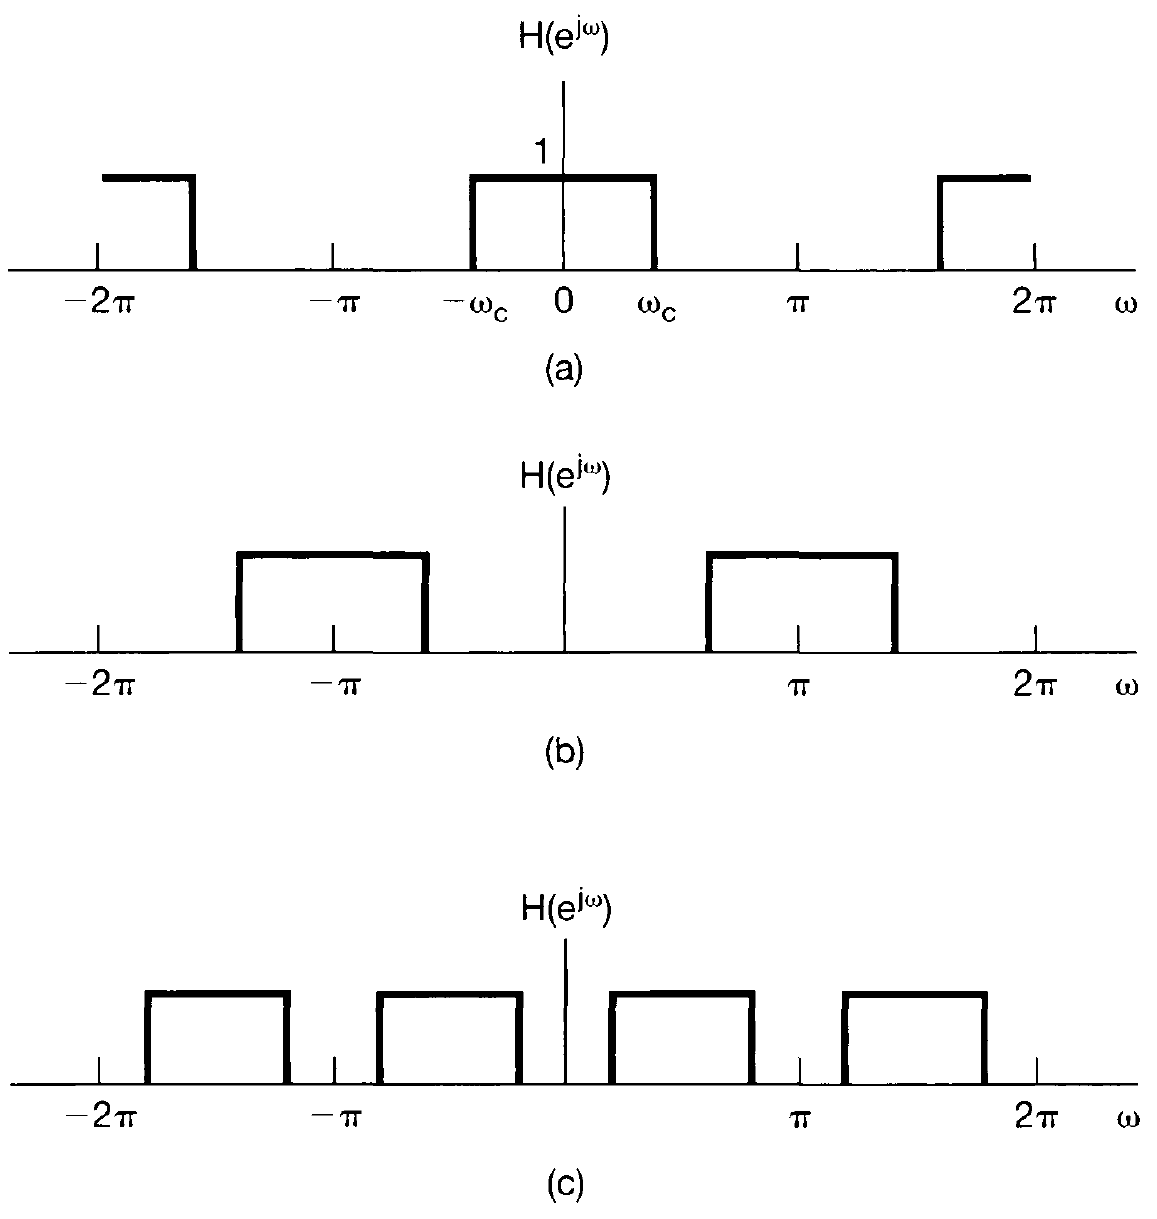
\includegraphics[width=0.3\textheight]{images/filters.png}

\section{Fourier Transform}

{\renewcommand{\arraystretch}{\stretchamt}
\begin{tabular}{@{}ll}
    Synthesis & $x(t)=\frac{1}{2\pi}\infint X(j\om)e^{j\om t}\d\om$ \\
    Analysis & $X(j\om)=\infint x(t)e^{-j\om t}\d t$ \\
    Impulse & $H(j\om)=\infint e^{-j\om\tau}h(t)\d t$ \\
    & $h(t)=\frac{1}{2\pi}\infint e^{j\om t}H(j\om)\d\om$ \\
    Impulse train & $X(j\om)=\infsum 2\pi c_k\delta(w-k\om_0)$
\end{tabular}}

% \subsection{Dirichlet Conditions}

% {\renewcommand{\arraystretch}{\stretchamt}
% \begin{tabular}{@{}ll}
%     1. $x(t)$ is single-valued \\
%     2. $x(t)$ is absolutely integrable \\
%     3. $x(t)$ has finite extrema in any finite interval \\
%     4. $x(t)$ has finite discontinuities in any finite interval
% \end{tabular}}

% $\implies$ Fourier transform converges to $x(t)$ where continuous, and half the jump where discontinuous.

\subsection{Fourier Transform Properties}

{\renewcommand{\arraystretch}{\stretchamt}
\begin{tabular}{@{}ll}
    Linear & $ax(t)+by(t)\ft aX(j\om)+bY(j\om)$ \\
    Time shift & $x(t-t_0)\ft e^{-j\om t_0}X(j\om)$ \\
    Time scale & $x(at)\ft\frac{1}{|a|}X\lrb{\frac{j\om}{a}}$ \\
    Time reversal & $x(-t)=X(-j\om)$ \\
    Conjugation & $x^*(t)\ft X^*(-j\om)$ \\
    Convolution & $y(t)=h(t)*x(t)\rightarrow Y(j\om)=H(j\om)X(j\om)$ 
\end{tabular}}

% For real $x(t)$:

% {\renewcommand{\arraystretch}{\stretchamt}
% \begin{tabular}{@{}ll}
%     Decomp & $x(t)=f_e(t)+f_o(t)$ \\
%     & $x_e(t)=\frac 12(x(t)+x(-t))$ \\
%     & $x_o(t)=\frac 12(x(t)-x(-t))$ \\
%     Transform & $\F(x(t))=\F(x_e(t))+\F(x_o(t))$ \\
%     & $\F(x_e(t))=\Re(X(j\om))$ \\
%     & $\F(x_o(t))=j\cdot\Im(X(j\om))$
% \end{tabular}}

\section{Differentiation and Integration}

{\renewcommand{\arraystretch}{\stretchamt}
\begin{tabular}{@{}ll}
    Magnitude & $\abs{Y(j\om)}=\abs{X(j\om)}\abs{H(j\om)}$ \\
    Phase & $\phase Y(j\om)=\phase X(j\om)+\phase H(j\om)$ \\
    Differentiation & $\dv{x(t)}{t}\ft j\om X(j\om)$ \\
    Integration & $\int_{-\infty}^t x(\tau)\d\tau\ft\frac{1}{j\om}X(j\om)+\pi X(0)\delta(\om)$ \\
    Unit impulse & $\delta(t)\ft 1$ \\
    Unit step & $u(t)\ft\frac{1}{j\om}+\pi\delta(\om)$ \\
    Generic ODE
\end{tabular}}

\tab $\sum_{k=0}^N\al_k\frac{d^ky(t)}{dt^k}=\sum_{k=0}^M\be_k\frac{d^kx(t)}{dt^k}$

\tab $H(j\om)=\frac{Y(j\om)}{X(j\om)}=\frac{\sum_{k=0}^M\be_k(j\om)^k}{\sum_{k=0}^N\al_k(j\om)^k}=\frac{\text{X coeffs}}{\text{Y coeffs}}$

\section{Filter Behavior}

{\renewcommand{\arraystretch}{\stretchamt}
\begin{tabular}{@{}ll}
    Step response & $s(t)=h(t)*u(t)=\int_{-\infty}^t h(\tau)\d\tau$ \\
    1st order & $T\dv{y(t)}{t}+y(t)=x(t)$ \\
    & $H(j\om)=\frac{1}{1+j\om T}$ \\
    & $s(t)=(1-e^{-t/T})u(t)$ \\
    2nd order & $\ddv{y(t)}{t}+2\ze\om_n\dv{y(t)}{t}+\om_n^2y(t)=\om_n^2x(t)$ \\
    & $H(j\om)=\frac{\om_n^2}{(j\om)^2+2\ze\om_n(j\om)+\om_n^2}$ \\
    & $H(j\om)=\frac{\om_n^2}{(j\om-c_+)(j\om-c_-)}$ \\
    & $c_\pm=-\ze\om_n\pm\om_n\sqrt{\ze^2-1}$ \\
     & $s(t)=\sqb{1+\frac{\om_n}{2\sqrt{\ze^2-1}}\lrb{\frac{e^{c_+t}}{c_+}-\frac{e^{c_-}t}{c_-}}}u(t)$ \\
\end{tabular}}

\section{DT Fourier Transform}

{\renewcommand{\arraystretch}{\stretchamt}
\begin{tabular}{@{}ll}
    Synthesis & $x[n]=\frac{1}{2\pi}\int_{2\pi}X(e^{j\om})e^{j\om n}\d\om$ \\
    Analysis & $X(e^{j\om})=\sum_{n=-\infty}^\infty x[n]e^{-j\om n}$ \\
    Convergence & $\sum_{n=-\infty}^\infty\abs{x[n]}<\infty$ or $\sum_{n=-\infty}^\infty\abs{x[n]}^2<\infty$ \\
    \rlap{Difference Equations}
\end{tabular}}

\tab $\sum_{k=0}^Na_ky[n-k]=\sum_{k=0}^Mb_kx[n-k]$

\tab $H(e^{j\om})=\frac{Y(e^{j\om})}{X(e^{j\om})}=\frac{\sum_{k=0}^M b_ke^{-j\om k}}{\sum_{k=0}^N a_ke^{-j\om k}}=\frac{\text{X coeffs}}{\text{Y coeffs}}$

\section{Sampling}

{\renewcommand{\arraystretch}{\stretchamt}
\begin{tabular}{@{}ll}
    Sampling & $p(t)=\infsum\delta(t-kT)$ \\
    & $x_p(t)=x(t)p(t)$ \\
    Impulse train & $P(j\om)=\frac{2\pi}{T}\infsum\delta(\om-k\om_s)$ \\
    Freq domain & $X_p(j\om)=\frac 1T\infsum X(j(\om-k\om_s))$ \\
    Nyquist rate & $\om_s\ge 2\om_M$
\end{tabular}}

\subsection{CT-DT Conversion}

{\renewcommand{\arraystretch}{\stretchamt}
\begin{tabular}{@{}ll}
    Freq resp & $X_d(e^{j\Om})=X_p(j\frac\Om T)=\frac 1T\infsum X_c(j\frac{\Om-2\pi k}{T})$
\end{tabular}}

\subsection{DT Sampling}

{\renewcommand{\arraystretch}{\stretchamt}
\begin{tabular}{@{}ll}
    Sampling & $p[n]=\infsum\delta[n-kN]$ \\
    & $x_p[n]=\begin{cases}
        x[n], & n\text{ multiple of }N \\
        0 & \text{otherwise}
    \end{cases}$ \\
    Impulse train & $P(e^{j\om})=\frac{2\pi}{N}\infsum\delta(\om-k\om_s)$ \\
    Freq domain & $X_p(j\om)=\frac 1N\sum_{k=0}^{N-1}X(e^{j(\om-k\om_s)})$ \\
    Decimation & $x_b[n]=x[nN]$ \\
    & $X_b(e^{j\om})=X_p(e^{j\frac \om N})$ \\
    Interpolation & add $N-1$ points between
\end{tabular}}

\subsection{Modulation}

{\renewcommand{\arraystretch}{\stretchamt}
\begin{tabular}{@{}ll}
    Modulation & $Y(j\om)=\frac{1}{2\pi}\infint X(j\theta)P(j(\om-\theta))d\theta$ \\
    Amplitude (AM) & $c(t)=e^{j(\om_c t+\theta_c)}$ \\
    Sinusoidal AM & $c(t)=\cos(\om_c t+\theta_c)$
\end{tabular}}

\section{Laplace Transform}

{\renewcommand{\arraystretch}{\stretchamt}
\begin{tabular}{@{}ll}
    Laplace & $X(s)=\infint x(t)e^{-st}\d t$ \\
    & $X(s)=\F\sqb{e^{-\sigma t}x(t)}\qquad s=\sigma+j\om$ \\
    % Right & $x(t)=e^{-at}u(-t)$ \\
    % & $\lt X(s)=\frac{1}{s+a},\quad \Re(s)>-a$ \\
    % Left & $x(t)=-e^{-at}u(-t)$ \\
    % & $\lt X(s)=\frac{1}{s+a},\quad \Re(s)<-a$
\end{tabular}}

{\renewcommand{\arraystretch}{\stretchamt}
\begin{tabular}{@{}ll}
    1. ROC no $j\om$ axis $\iff$ FT does not converge \\
    2. ROC of rational $\L$ contains no poles \\
    3. $x(t)$ finite duration and absolutely integrable \\
    $\hspace{2ex}\implies$ ROC = s-plane \\
    4. $x(t)$ left sided and $\Re(s)=\sigma_0$ in ROC \\
    $\hspace{2ex}\implies$ $s \text{ s.t. } \Re(s)<\sigma_0$ in ROC \\
    5. $x(t)$ right sided and $\Re(s)=\sigma_0$ in ROC \\
    $\hspace{2ex}\implies$ $s \text{ s.t. } \Re(s)>\sigma_0$ in ROC \\
    6. $x(t)$ two sided, then ROC is a strip or does not exist
\end{tabular}}

\subsection{Laplace Transform Properties}

{\renewcommand{\arraystretch}{\stretchamt}
\begin{tabular}{@{}ll}
    Linear & $ax_1(t)+bx_2(t)\lt aX_1(s)+bX_2(s)$ \\
    & $\ROC \supseteq R_1\cap R_2$ \\
    Time shift & \twoEqn{x(t-t_0)\lt e^{-st_0}X(s)}{\ROC=R}{12em}{5em} \\
    Time scale & \twoEqn{x(at)\lt\frac{1}{|a|}X\lrb{\frac{s}{a}}}{\ROC=aR}{12em}{5em} \\
    Time reversal & \twoEqn{x(-t)=X(-s)}{\ROC=-R}{12em}{5em} \\
    Differentiation & \twoEqn{\dv{x(t)}{t}\lt sX(s)}{\ROC\supseteq R}{12em}{5em} \\
    & \twoEqn{-tx(t)\lt\dv{X(s)}{s}}{\ROC=R}{12em}{5em} \\
    Conjugation & \twoEqn{x^*(t)\lt X^*(-s^*)}{\ROC=R}{12em}{5em} \\
    Convolution & $x_1(t)*x_2(t)\lt X_1(s)X_2(s)$ \\
    & $\ROC \supseteq R_1\cap R_2$ \\
\end{tabular}}

\subsection{Systems}

{\renewcommand{\arraystretch}{\stretchamt}
\begin{tabular}{@{}ll}
    Causal & ROC is a right-half plane \\
    Stable & for rational $H(s)$, stable iff ROC contains $j\om$ \\
    & and there aren't more zeros than poles \\
    ODE &
\end{tabular}}

\tab $\sum_{k=0}^N\al_k\frac{d^ky(t)}{dt^k}=\sum_{k=0}^M\be_k\frac{d^kx(t)}{dt^k}$

\tab $H(s)=\frac{Y(s)}{X(s)}=\frac{\sum_{k=0}^M\be_ks^k}{\sum_{k=0}^N\al_ks^k}=\frac{\text{X coeffs}}{\text{Y coeffs}}$

\# of zeros at infinity = deg($D$)-deg($N$)

\section{Feedback Systems}

\subsection{Feedback}

\tab 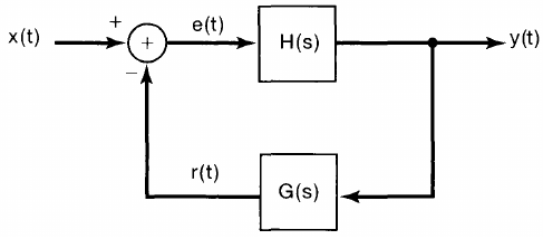
\includegraphics[width=0.2\textwidth]{images/feedback.png}

\tab $Q(s)=\frac{H(s)}{1+G(s)H(s)}$

\subsection{Inverse}

\tab 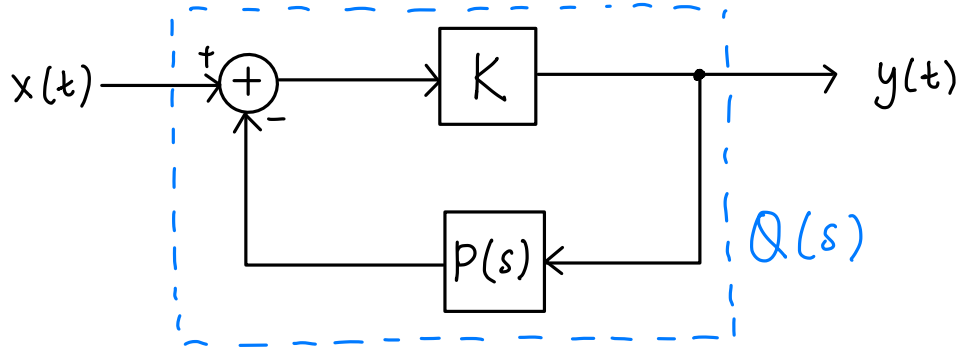
\includegraphics[width=0.2\textwidth]{images/feedback_inverse.png}

\tab $Q(s)=\frac{K}{1+KP(s)}\approx\frac{1}{P(s)}$ for large $K$

\subsection{Stabilize}

\tab 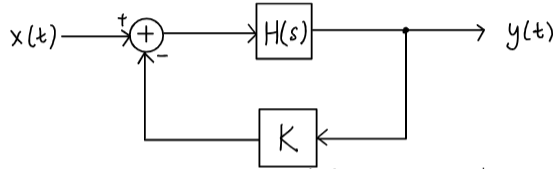
\includegraphics[width=0.2\textwidth]{images/feedback_stabilize.png}

\tab $H(s)=\frac{b}{s-a}\implies Q(s)=\frac{b}{s-a+Kb}$. Stable if $K>\frac ab$

\section{Z Transform}

{\renewcommand{\arraystretch}{\stretchamt}
\begin{tabular}{@{}ll}
    Transform & $X(z)=\sum_{n=-\infty}^\infty x[n]z^{-n}$ \\
    Feedback & $Q(z)=\frac{H(z)}{1+H(z)G(z)}$
\end{tabular}}

\tab 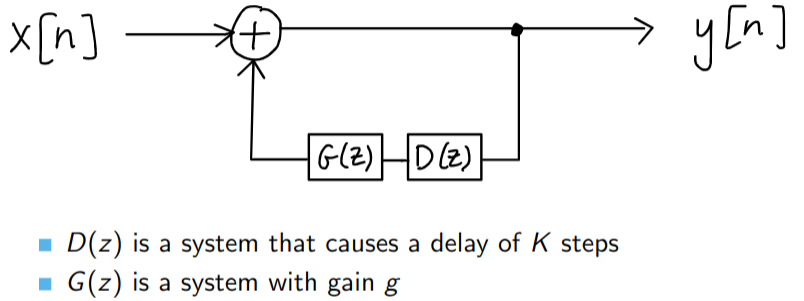
\includegraphics[width=0.2\textwidth]{images/comb.png}

$Q(z)=\frac{z^k}{z^k-g}$

\section{Miscellaneous}

{\renewcommand{\arraystretch}{\stretchamt}
\begin{tabular}{@{}ll}
    Geometric & $\sum_{k=0}^N a^k=\frac{1-a^{N+1}}{1-a}$ 
\end{tabular}}


\rule{\linewidth}{0.1pt}
{\scriptsize 
Compiled \today}

\end{multicols*}

\begin{multicols*}{2}

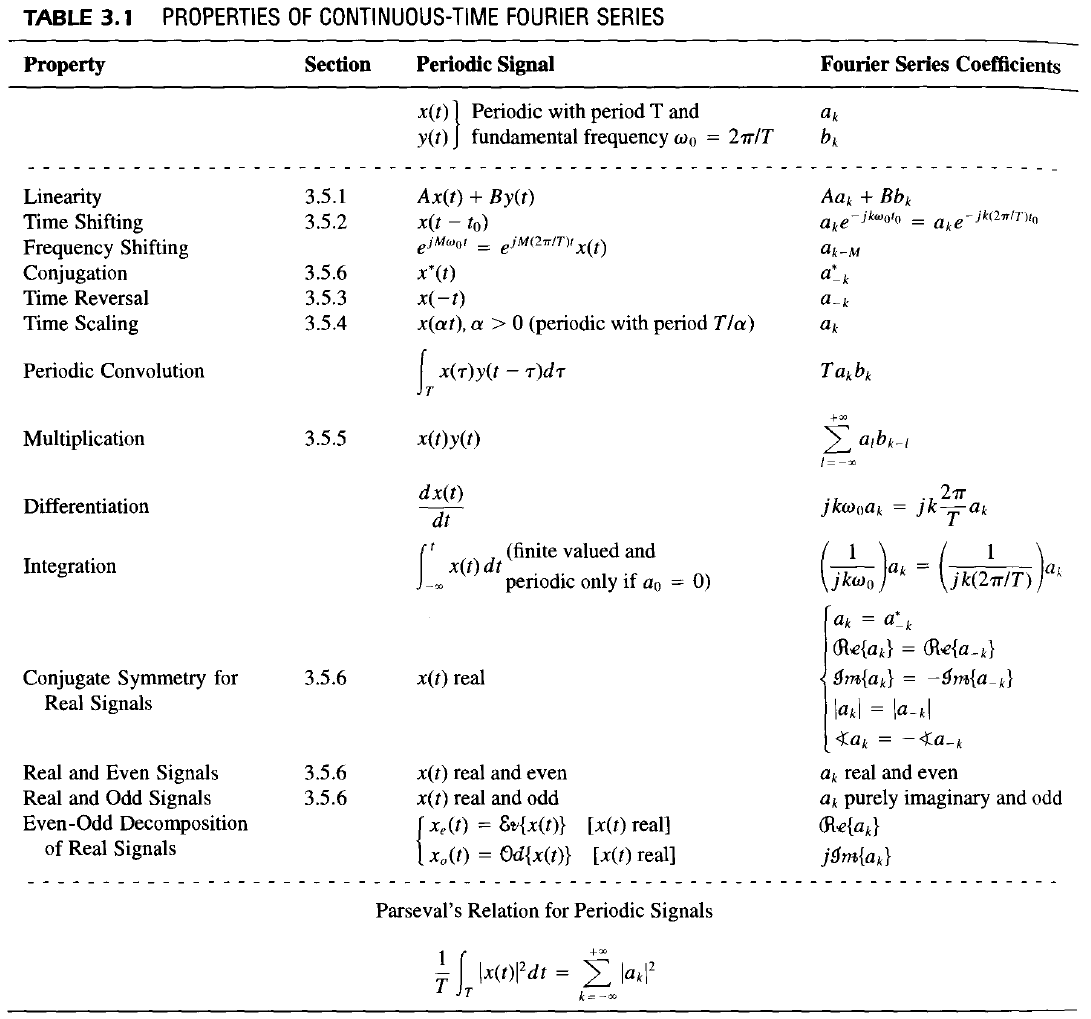
\includegraphics[width=\tablewidth]{images/CT_fourier_series_properties.png}

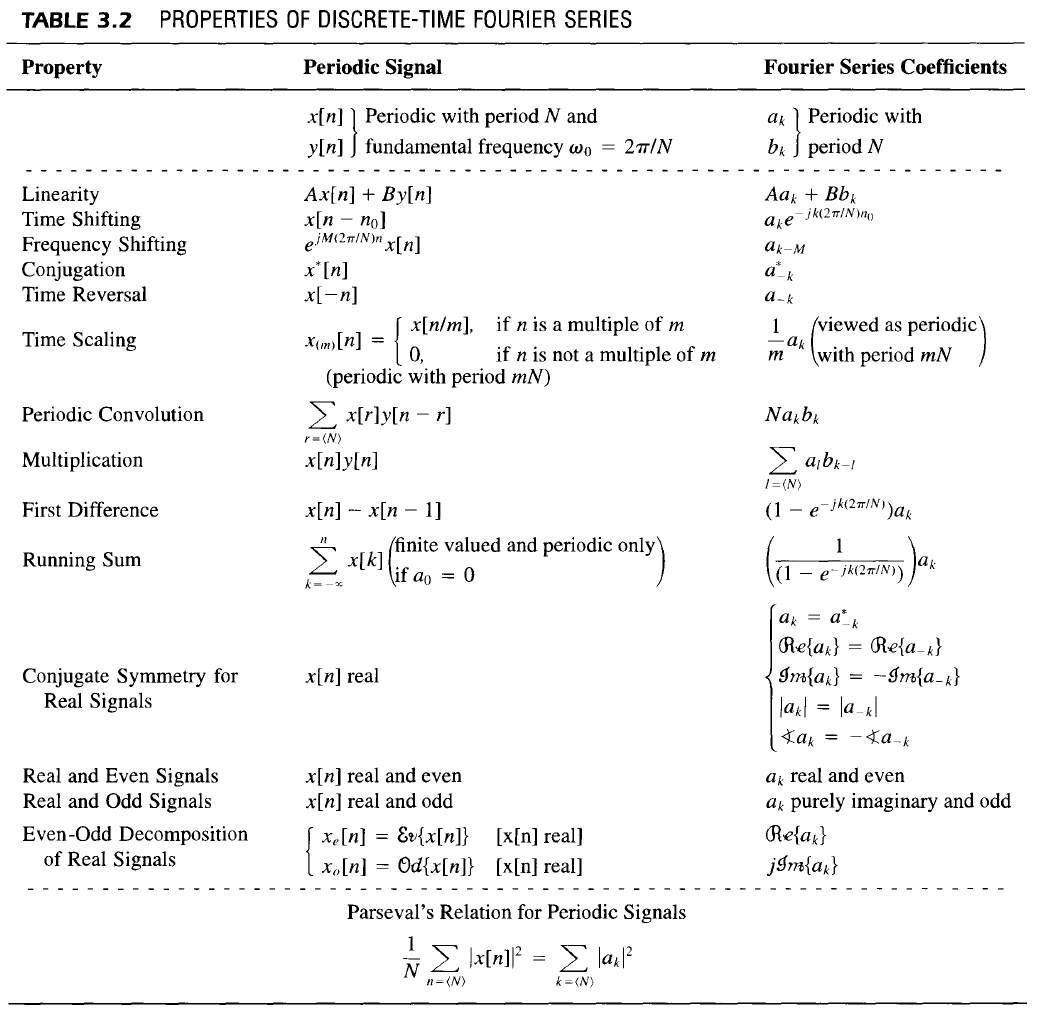
\includegraphics[width=\tablewidth]{images/DT_fourier_series_properties.png}

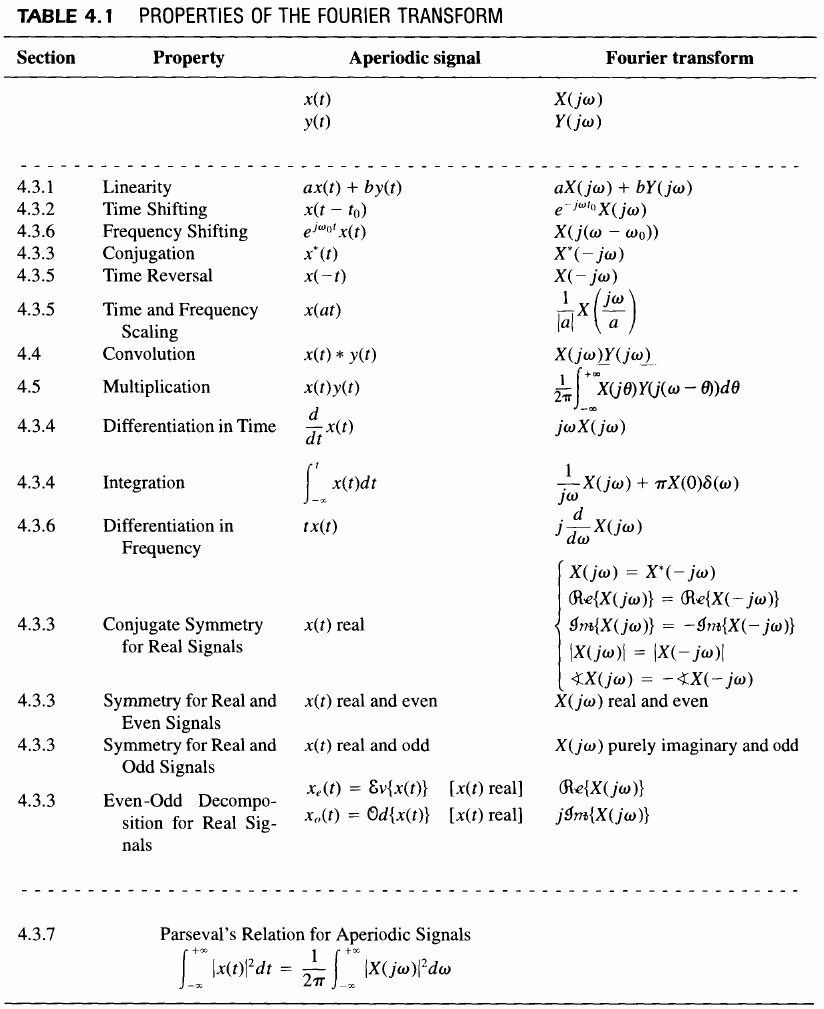
\includegraphics[width=\tablewidth]{images/CT_fourier_transform_properties.png}

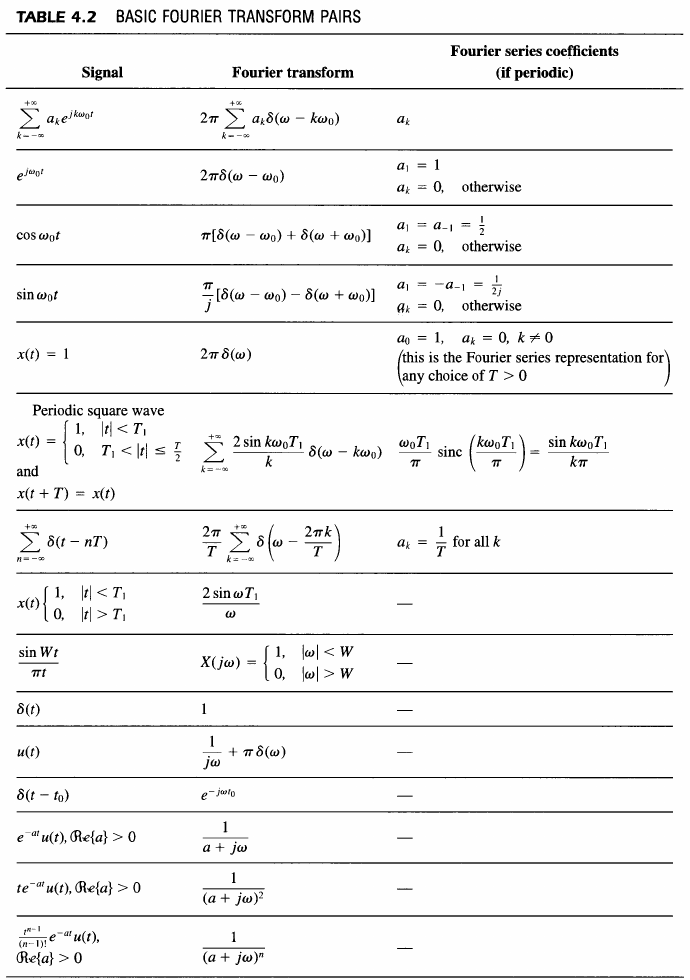
\includegraphics[width=\tablewidth]{images/CT_fourier_transform_pairs.png}

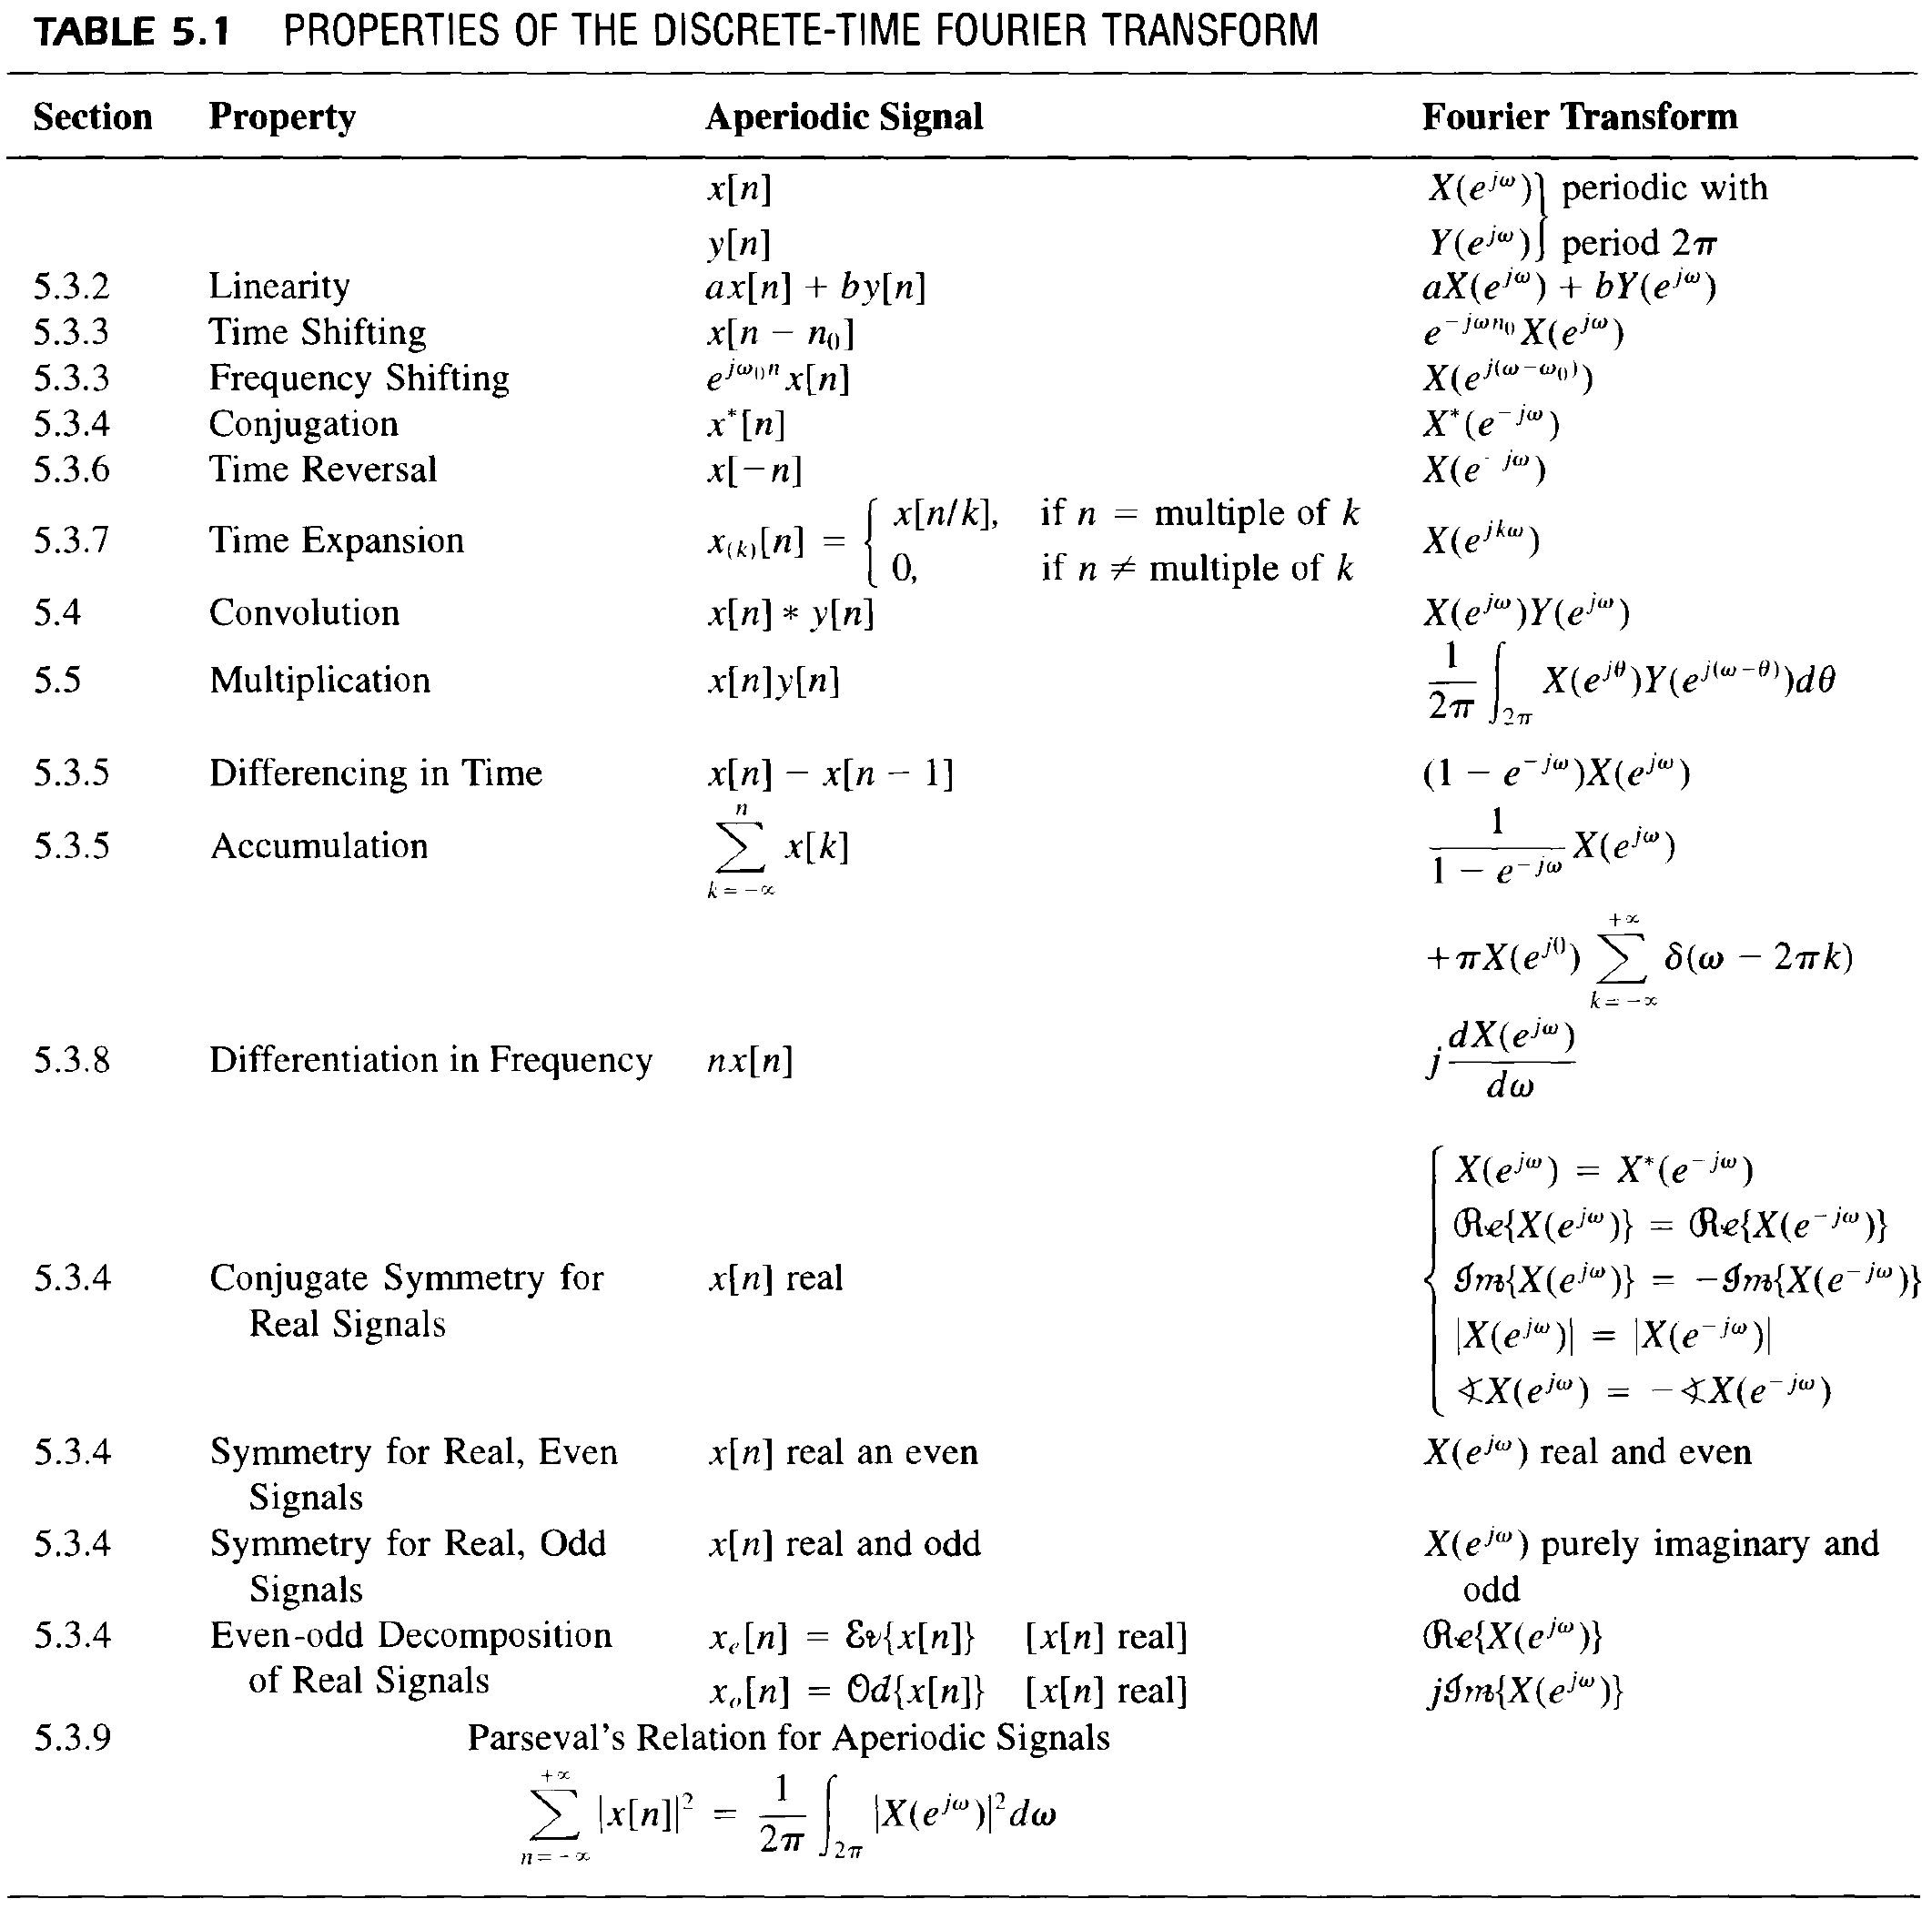
\includegraphics[width=\tablewidth]{images/DT_fourier_transform_properties.png}

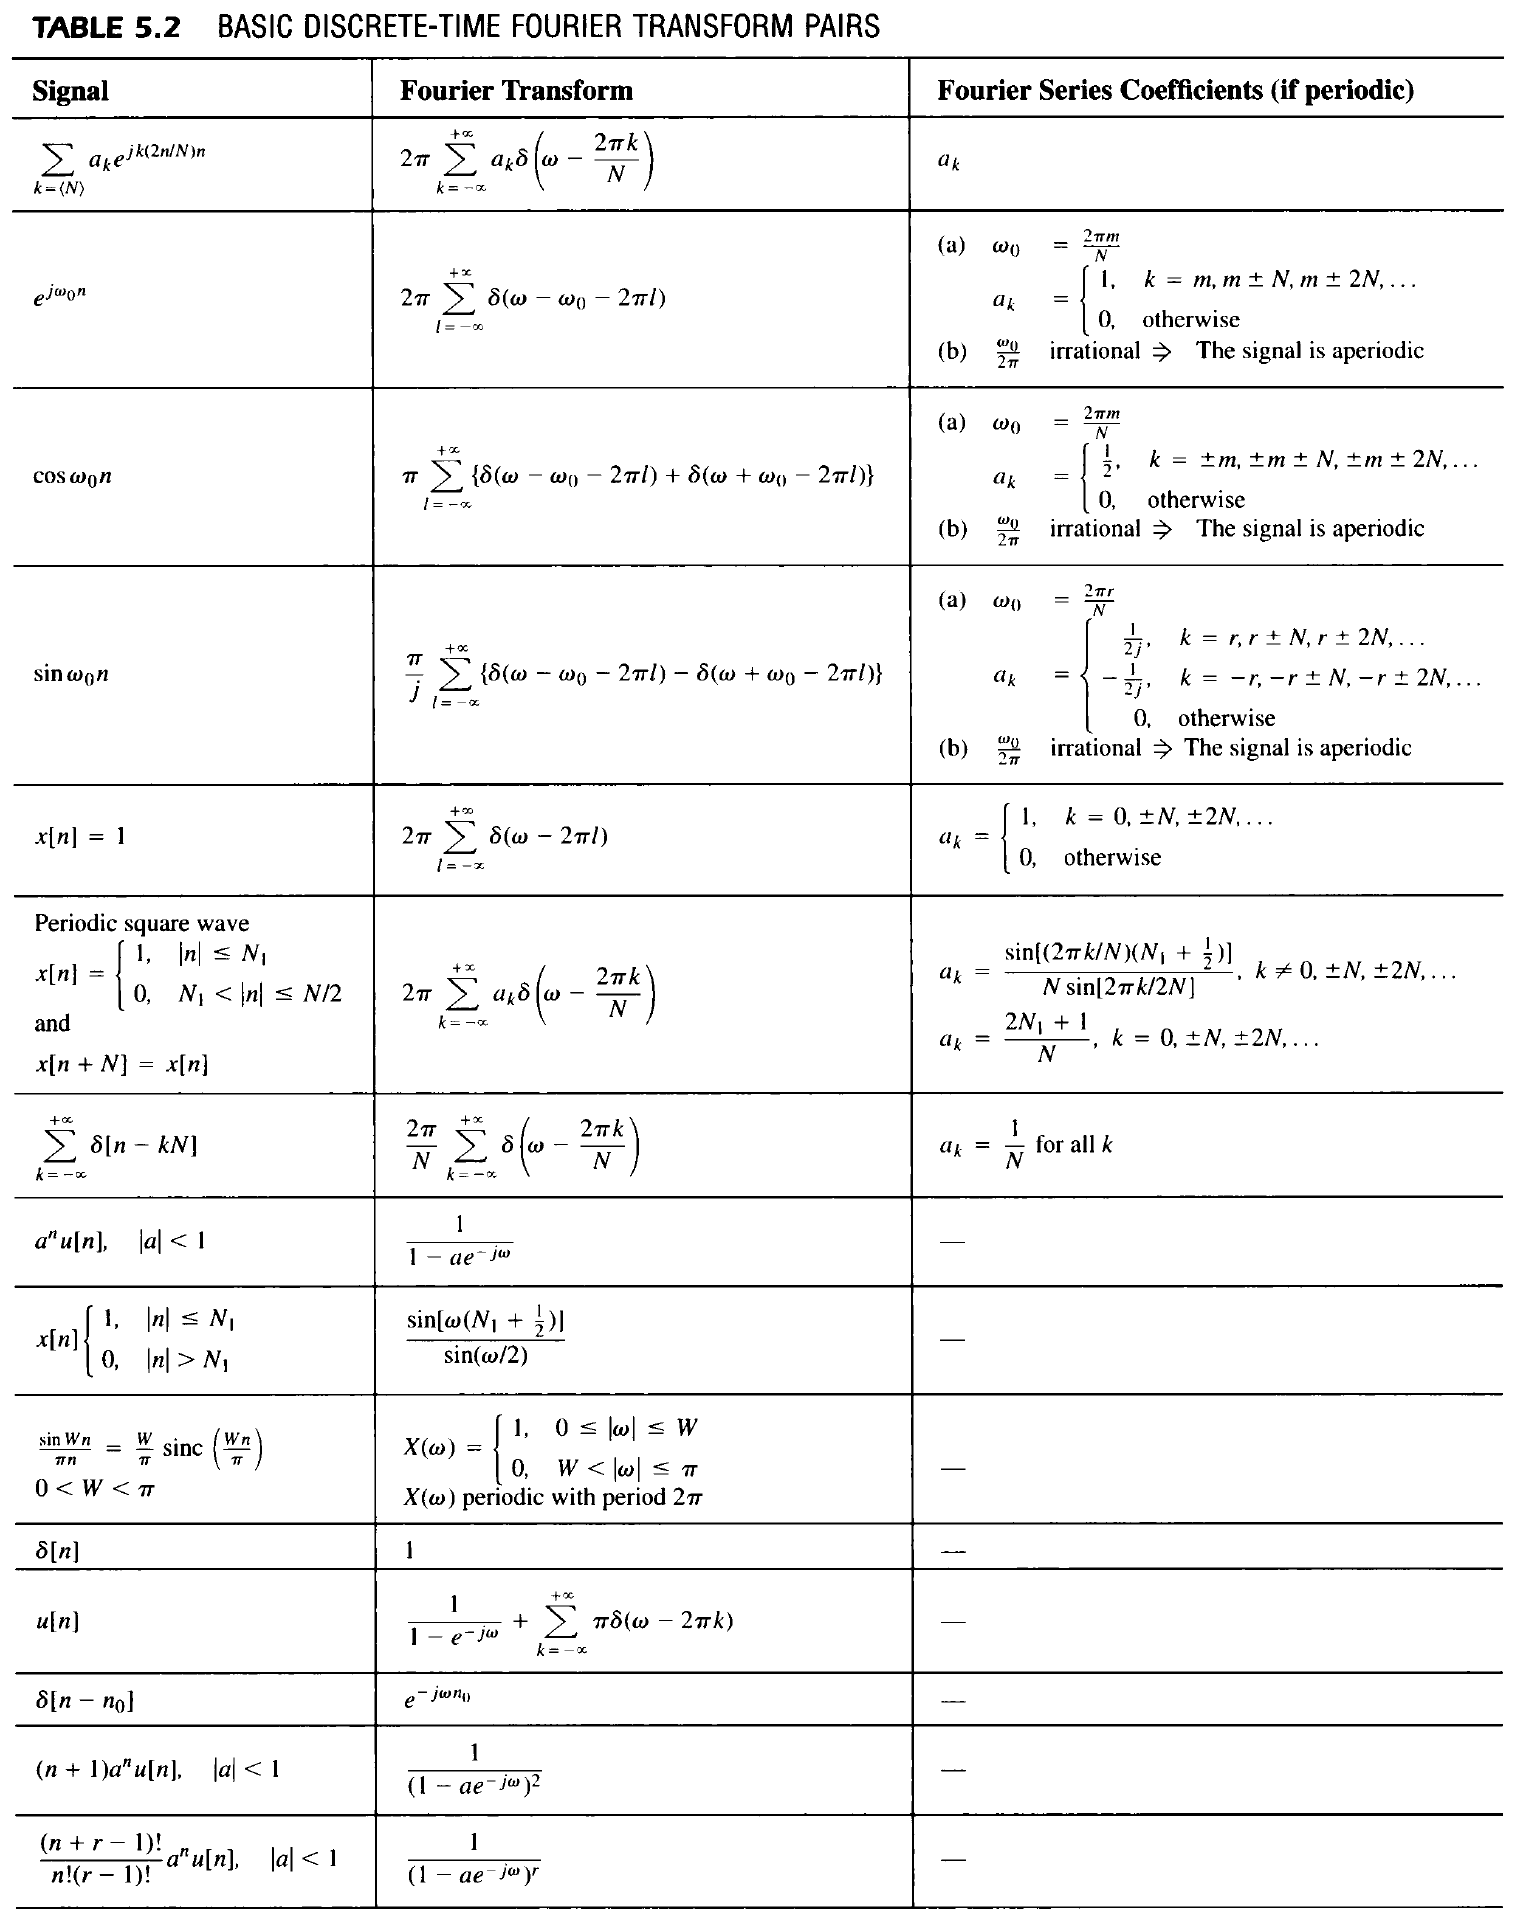
\includegraphics[width=\tablewidth]{images/DT_fourier_transform_pairs.png}

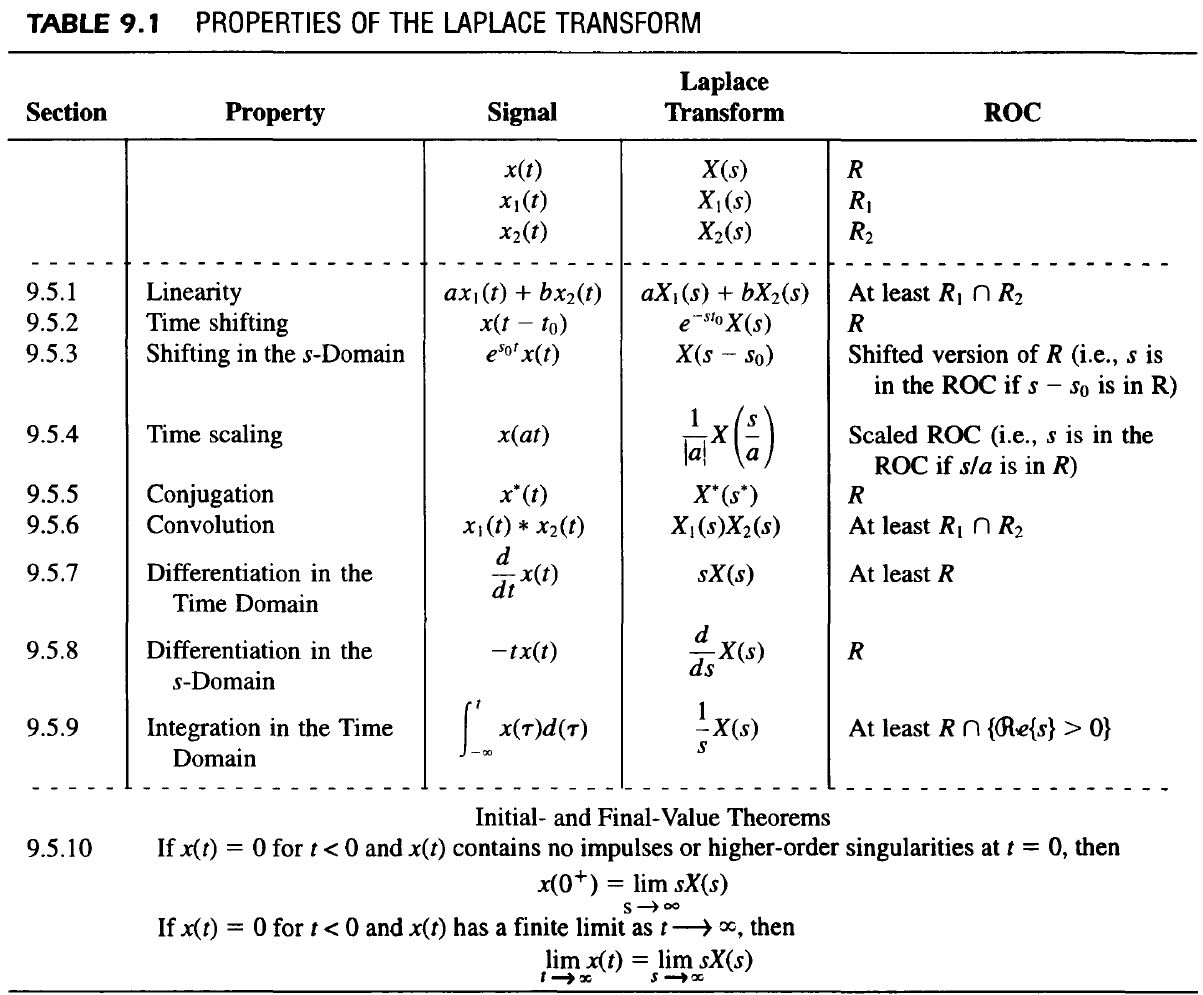
\includegraphics[width=\tablewidth]{images/Laplace_properties.png}

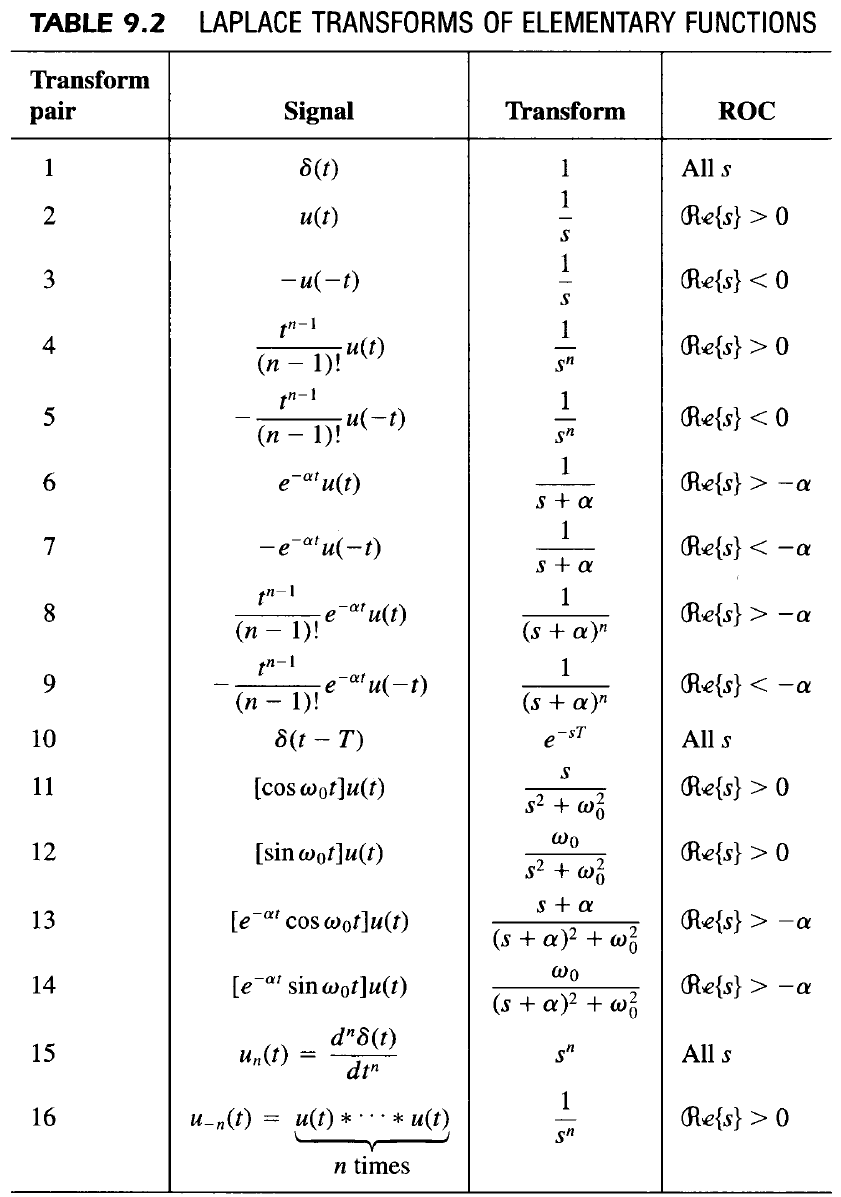
\includegraphics[width=0.35\textwidth]{images/Laplace_pairs.png}

\end{multicols*}

\end{document}